\begin{frame}
  \frametitle{Ce este Învățarea Automată?}
  \begin{block}{Învățarea automată}
    Un program se spune că învață dintr-o mulțime de experiențe $E$
    relativ la o clasă de task-uri $T$ și o măsură a performanței $P$
    dacă performanța acestuia la execuția task-urilor $T$, măsurată de $P$,
    se îmbunătățește în urma experiențelor $E$.
    \citep{Mitchell:1997:ML:541177}
  \end{block}
\end{frame}

\begin{frame}[t]
  \frametitle{Aplicații ale Învățării Automate}
  \begin{itemize}
  \item \alert<1>{Self-Driving Car: Google Car}
  \item \alert<2>{Traducere Automată: Google Translate}
  \item \alert<3->{Sisteme de Recomandare}
    \begin{itemize}
    \item \alert<3>{Filme: ImDB, NetFlix}
    \item \alert<4>{Publicitate Inteligentă: Google Ads, Facebook Ads}
    \end{itemize}
  \end{itemize}
  \begin{center}%
    \only<1>{%
      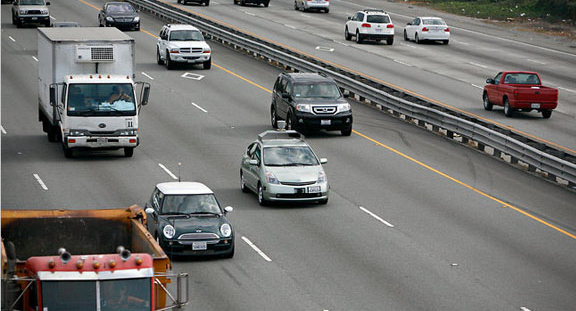
\includegraphics[width=0.45\textwidth]{graphics/ml-intro/google-car-2}%
      \hspace*{2em}%
      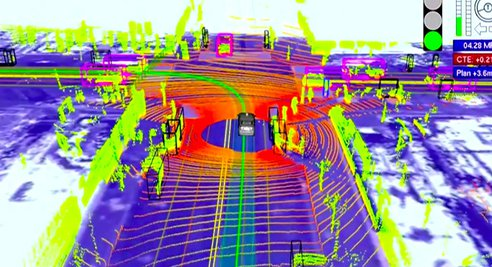
\includegraphics[width=0.45\textwidth]{graphics/ml-intro/google-car}%
      \newline%
      {\scriptsize imagini de pe \url{www.nytimes.com}}
    }%
    \only<2>{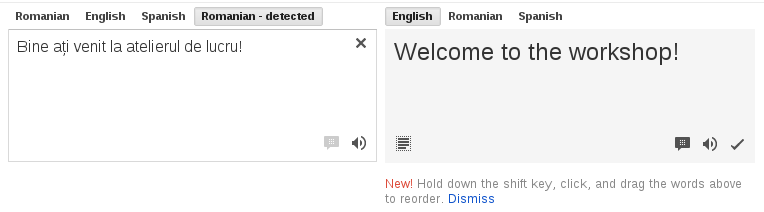
\includegraphics[width=0.9\textwidth]{graphics/ml-intro/translate}}%
    \only<3>{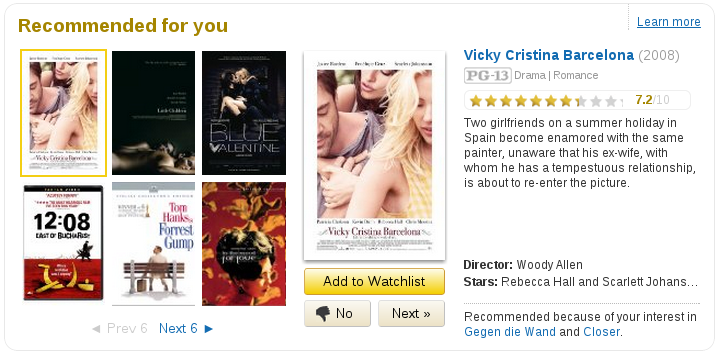
\includegraphics[width=0.65\textwidth]{graphics/ml-intro/recommender}}%
    \only<4>{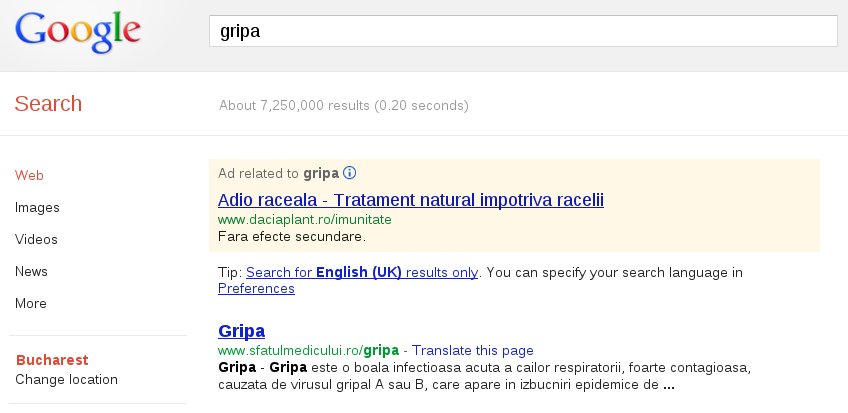
\includegraphics[width=0.65\textwidth]{graphics/ml-intro/gripa}}%
  \end{center}
\end{frame}

\begin{frame}[t]
  \frametitle{Învățarea Automată: Tipuri de probleme}
  \begin{block}{Tipuri de probleme}
    \begin{itemize}
    \item Regresie
      \begin{itemize}
      \item predicția evoluției prețului unui bun
      \end{itemize}%
      \item Clasificare
        \begin{itemize}
        \item clasificarea obiectelor dintr-o imagine
        \end{itemize}
    \end{itemize}
  \end{block}%
  \begin{center}
    \only<1>{
\includegraphics[width=.5\textwidth]{graphics/ml-intro/ml-1}}%
    \only<2>{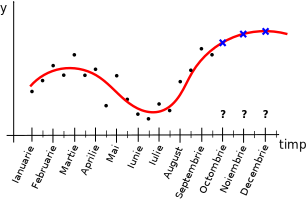
\includegraphics[width=.5\textwidth]{graphics/ml-intro/ml-2}}%
    \only<3>{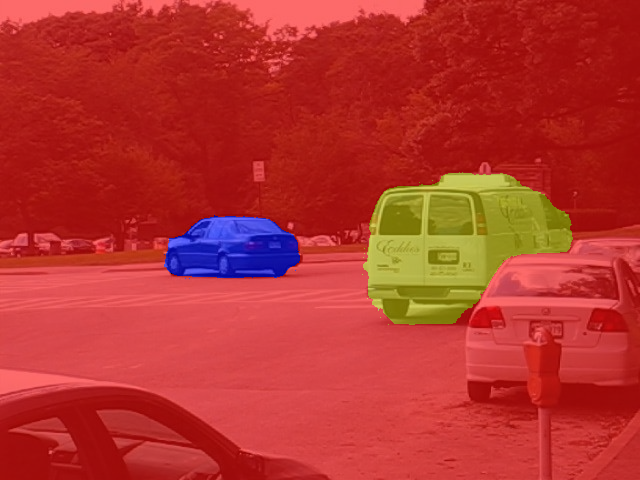
\includegraphics[width=.38\textwidth]{graphics/ml-intro/car-2}}%
    \only<4>{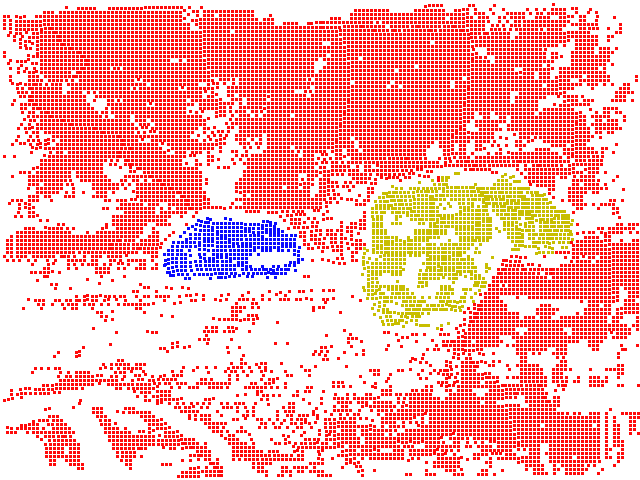
\includegraphics[width=.38\textwidth]{graphics/ml-intro/car-1}}%
    \only<3-4>{\\{\scriptsize imagine de la Albert-Ludwigs-Universität,\\ 
        Lehrstuhl für Mustererkennung und Bildverarbeitung}}%
    %\only<5>{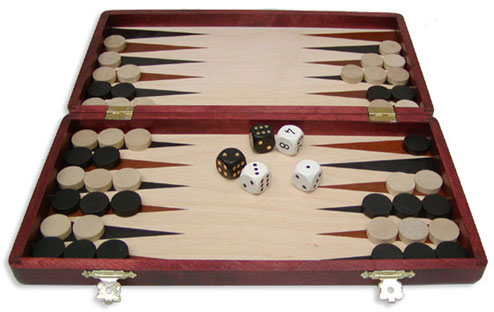
\includegraphics[width=.28\textwidth]{graphics/ml-intro/backgammon}}%
  \end{center}
\end{frame}

\begin{frame}
  \frametitle{Tipuri de învățare}
  \begin{block}{Învățare Supervizată}
    \alert{Învățarea supervizată} se face pe baza unor date de antrenare etichetate.
    \begin{itemize}
    \item construirea unui model climatic pe baza datelor din utimii 30 de ani
    \item construirea unui detector de mesaje spam
    \end{itemize}
  \end{block}\pause
  \begin{block}{Învățare Nesupervizată}
    În \alert{învățarea nesupervizată} nu există date etichetate.
    \begin{itemize}
    \item detectarea profilurilor de comportament ale cumpărătorilor
    \end{itemize}
  \end{block}\pause
  \begin{block}{Învățare prin Recompensă}
    În \alert{învățarea prin recompensă} un \emph{agent} caută să execute acele
    acțiuni are îi aduc o recompensă mai mare din partea mediului.
    \begin{itemize}
    \item inteligența artificială pentru jocuri
    \end{itemize}
  \end{block}  
\end{frame}